\chapter{Rezultaty pomiarów}
Testy całego systemu pomiarowego zostały przeprowadzone w dwóch różnych środowiskach. W pierwszym przypadku mierzone były warunki atmosferyczne panujące na zewnątrz budynku mieszkalnego. Drugi test został przeprowadzony we wnętrzu budynku.
\section{Warunki zewnętrzne}
Cały układ pomiarowy został testowo wykorzystany do badania warunków  meteorologicznych panujących na wolnym powietrzu. Aplikacja zbierająca dane została uruchomiona na kilka godzin (od około 15:00 do 21:00).

Poniższe wykresy prezentują warunki wtedy panujące. Jak widać na załączonych rysunkach, temperatura stale maleje wraz z upływem czasu. Świadczy to o poprawnym pomiarze, gdyż wraz z zachodzącym słońcem, robi się coraz chłodniej.
\begin{figure}[h!]
\centering
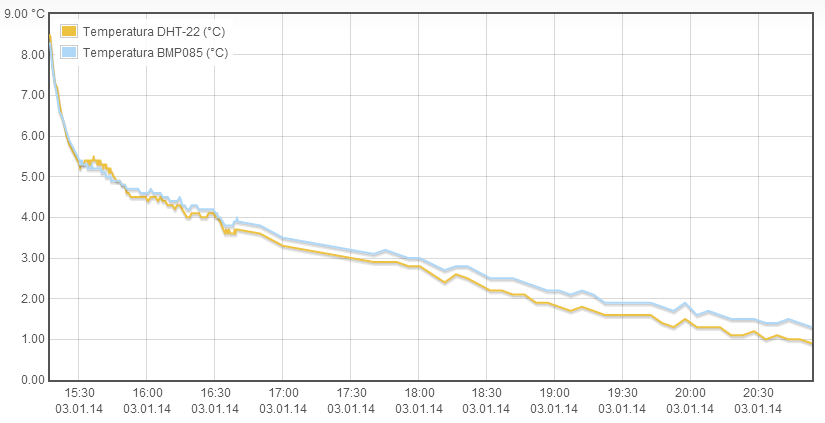
\includegraphics[scale=0.7]{zewnatrz_temp}
\caption{Pomiar temperatury na zewnątrz budynku}
\label{fig:zewnatrz_temp}
\end{figure}

Na wykresie \ref{fig:zewnatrz_temp} można zaobserwować stałą różnicę pomiędzy wskazaniami temperatur pomiędzy czujnikami DHT-22 oraz BMP085. Różnice w ich pomiarach wynoszą około 0,5 do 1 stopnia celsjusza i są spowodowane różnymi dokładnościami urządzeń mierzących.

Rysunek \ref{fig:zewnatrz_reszta} przedstawia zależności wilgotności powietrza oraz ciśnienia atmosferycznego od czasu, w którym następowało badanie.
\begin{figure}[h!]
\centering
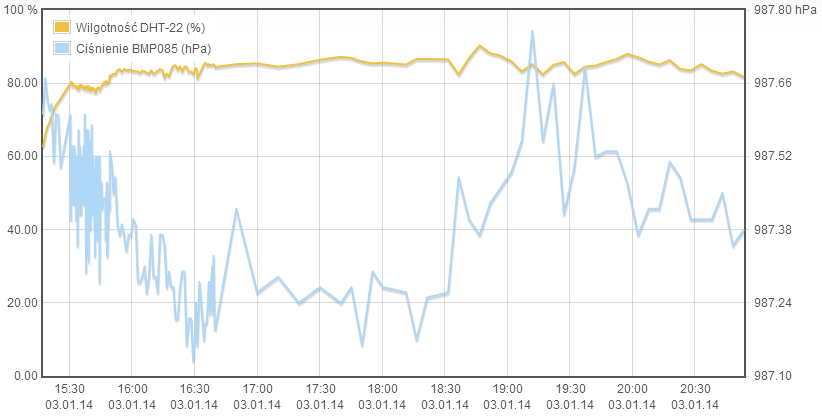
\includegraphics[scale=0.7]{zewnatrz_reszta}
\caption{Pomiar wilgotności oraz ciśnienia na zewnątrz budynku}
\label{fig:zewnatrz_reszta}
\end{figure}

Wahania ciśnienia atmosferycznego widoczne na wykresie \ref{fig:zewnatrz_temp} spowodowane są zakłóceniami w systemie pomiarowym oraz dokładnością czujnika.

\section{Warunki pokojowe}
Następnie stacja pogodowa została ustawiona w pokoju, gdzie temperatura nie ulega dużym wahaniom i uruchomiono aplikacją zbierającą pomiary. Wykres na rysunku \ref{fig:wewnatrz_temp} przedstawia zależność temperatur od czasu, natomiast rysunek \ref{fig:wewnatrz_reszta} prezentuje pomiary ciśnienia atmosferycznego oraz wilgotności.
\begin{figure}[h]
\centering
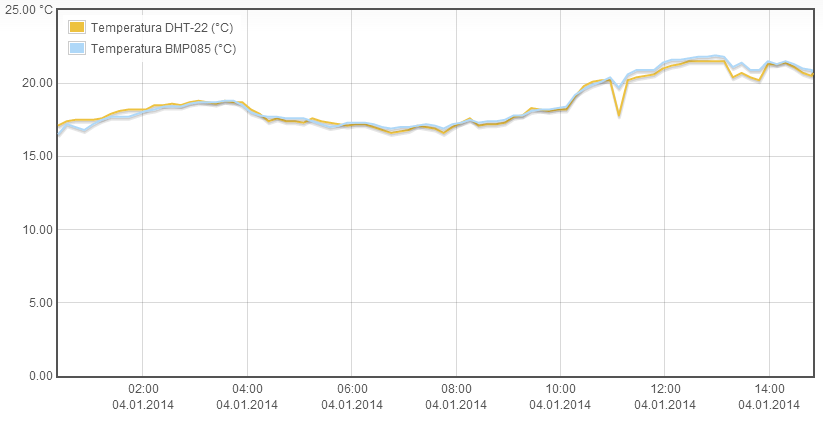
\includegraphics[scale=0.7]{wewnatrz_temp}
\caption{Pomiar temperatury wewnątrz pomieszczenia}
\label{fig:wewnatrz_temp}
\end{figure}
Jak można zauważyć z wykresu temperatur, w nocy miała ona stosunkowo niską wartość, natomiast nad ranem zaczeła rosnąć. Wiąże się to z faktem otwarcia okna oraz chłodzenia pomieszczenia, w celu uzyskania lepszego wypoczynku podczas snu oraz zamknięcia okna nad ranem.

\begin{figure}[h]
\centering
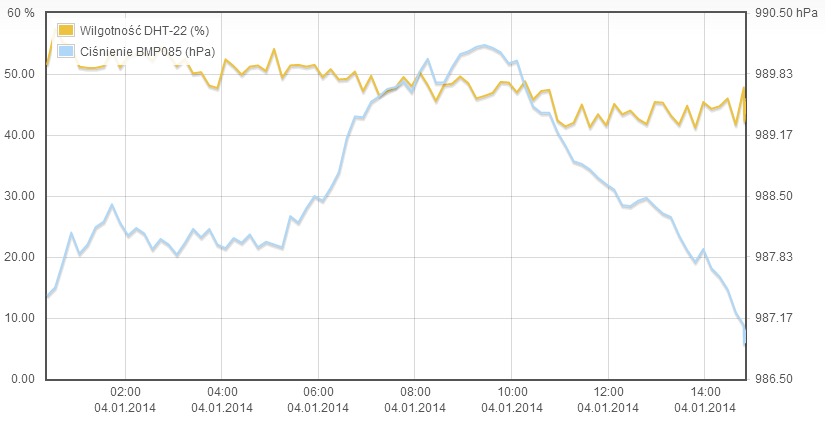
\includegraphics[scale=0.7]{wewnatrz_reszta}
\caption{Pomiar wilgotności oraz ciśnienia wewnątrz pomieszczenia}
\label{fig:wewnatrz_reszta}
\end{figure}